\chapter{Introducción}

\section{¿Qué es un fractal?}

La definición más inmediata que tenemos de los fractales es la siguiente:

\begin{definition}
    Un fractal es un objeto geométrico cuya estructura básica, fragmentada o irregular, se repite a diferentes escalas.
\end{definition}

\noindent Que su estructura básica se repita a diferentes escalas significa que el objeto es autosimilar.

\section{Autosimilitud}

Benoît Mandelbrot la definió como sigue:

\begin{definition}
    Un objeto es autosimilar o autosemejante si sus partes tienen la misma forma o estructura que el todo, aunque pueden presentarse a diferente escala y pueden estar ligeramente deformadas.
\end{definition}

\noindent
\large Vamos a ver dos tipos de autosimilitud:

\subsection{Autosimilitud exacta}

\begin{definition}
    Un objeto es exactamente autosimilar si es exactamente igual a sí mismo a diferentes escalas..
\end{definition}

\noindent
Es la más restrictiva de todas y la que vemos en los fractales clásicos. Algunos ejemplos de objetos exactamente autosimilares son:

\begin{itemize}
    \item El triángulo de Sierpinski
    
    \begin{figure}[H]
        \centering
        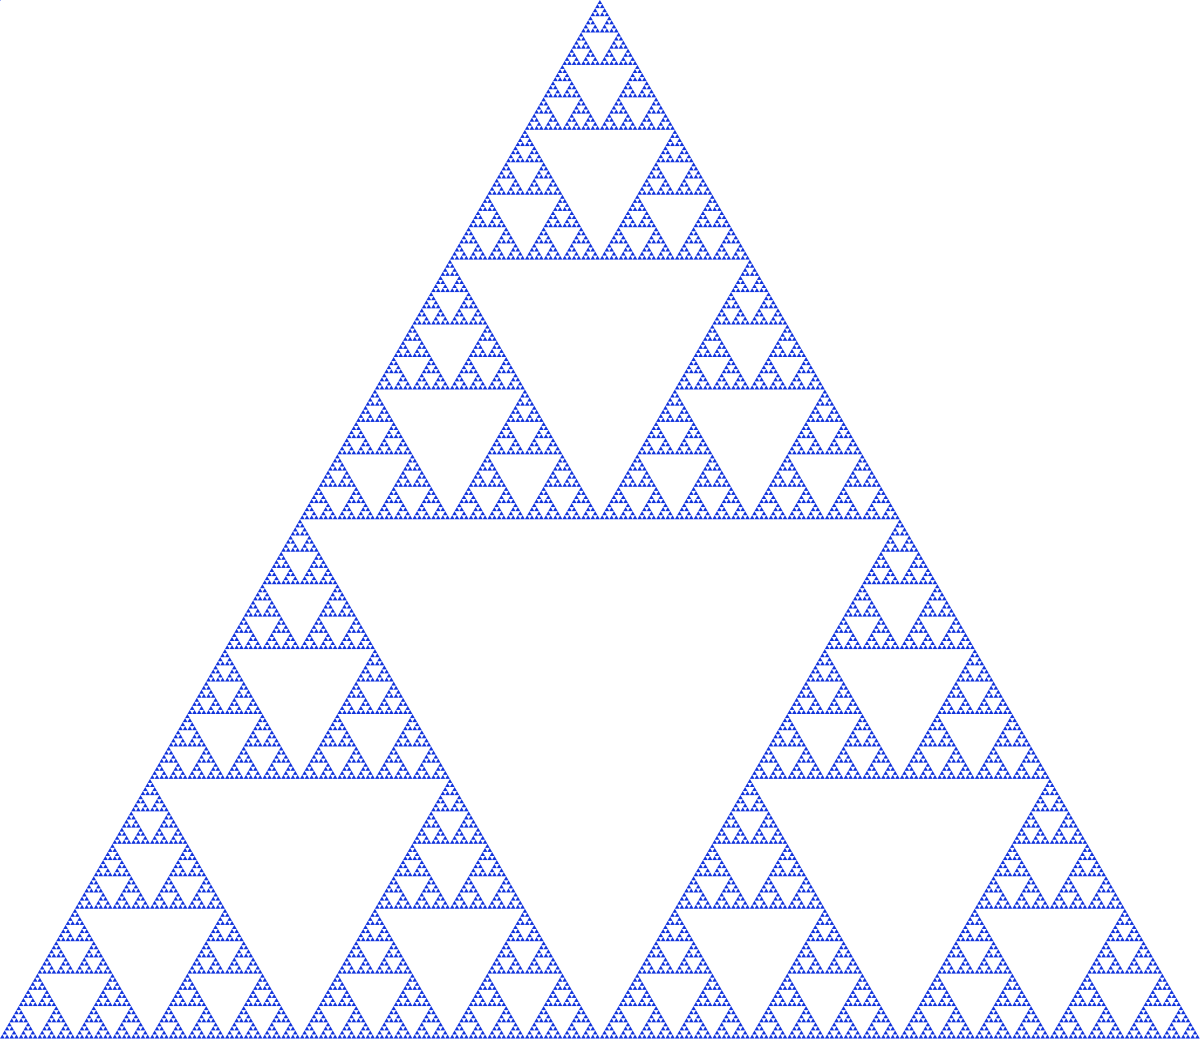
\includegraphics[width=0.5\textwidth]{figures/sierpinski-triangle.png}
        \caption{Triángulo de Sierpinski}
    \end{figure}

    \item El copo de Koch
    
    \begin{figure}[H]
        \centering
        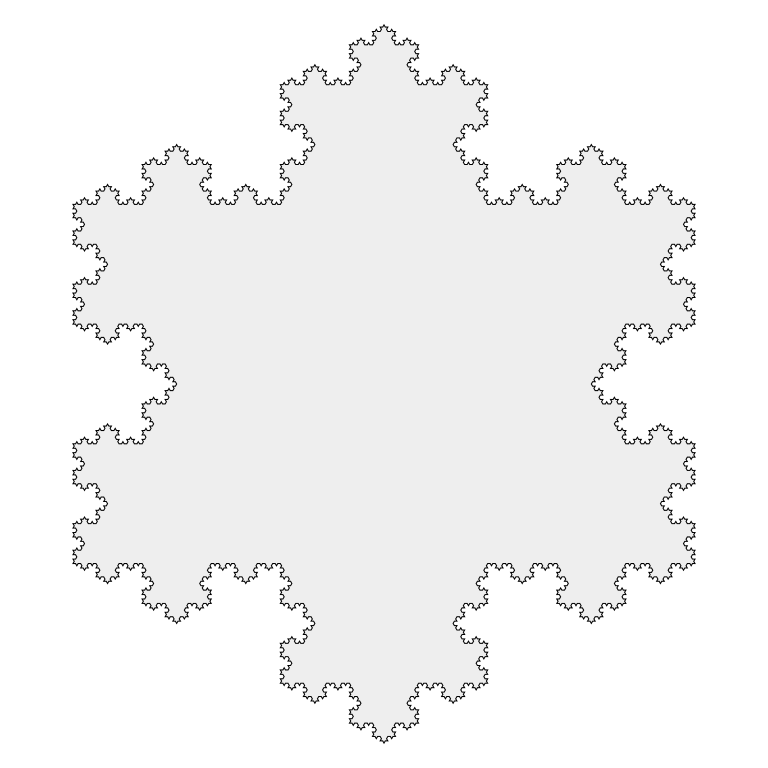
\includegraphics[width=0.5\textwidth]{figures/koch-snowflake.png}
        \caption{Copo de Koch}
    \end{figure}

\end{itemize}

\subsection{Cuasiautosimilitud}

\begin{definition}
    Un objeto es cuasiautosimilar si es aproximadamente igual a sí mismo a diferentes escalas.
\end{definition}

\noindent
Los fractales de este tipo contienen copias menores y distorsionadas de si mismos, como occure por ejemplo con el conjunto de Mandelbrot.

\begin{figure}[H]
    \centering
    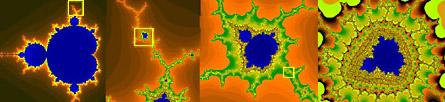
\includegraphics[width=0.7\textwidth]{figures/mandelbrot-cuasi.png}
    \caption{Ejemplos de cuasiautosimilitud en el conjunto de Mandelbrot}
\end{figure}


\section{Definición más formal}

\noindent En 1982 Benoît Mandelbrot definió los fractales de la siguiente forma:

\begin{definition}
Un fractal es un conjunto cuya dimensión de Hausdorff-Besicovitch es estrictamente mayor que su dimensión topológica.
\end{definition}

\noindent La dimensión topológica es la dimensión que todos conocemos, la dimensión de Hausdorff-Besicovitch es una de las formas de calcular la dimensión fractal de un objeto. 

\section{Dimensión fractal}

\noindent La dimensión fractal es una medida de la complejidad de un objeto fractal. La dimensión topológica de un objeto es un número entero, mientras que la dimensión fractal es un número real. La dimensión fractal es una generalización de la dimensión topológica.

\subsection{Cálculo de la dimensión fractal}

\noindent Ya hemos visto que una de las formas de calcular la dimensión fractal de un objeto es la dimensión de Hausdorff-Besicovitch, sin embargo esta resulta algo compleja. Otra forma más sencilla es con el método de \textit{Box Counting} también llamado o también conocido como la dimensión de Minkowski-Bouligard.\\

\noindent Para entender mejor este método vamos a verlo con un ejemplo. Consideremos un segemento y el borde de un cuadrado ambos de lado $1$.

\begin{figure}[H]
    \centering
    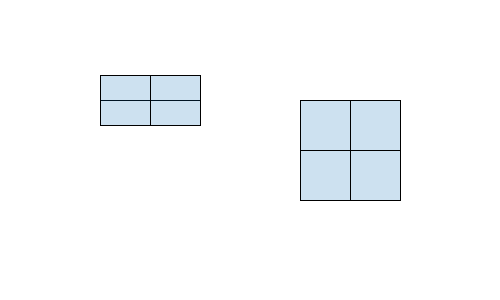
\includegraphics[width=0.7\textwidth]{figures/boxcounting-1.png}
    \caption{Box Counting - Cajas de lado $\frac{1}{2}$}
\end{figure}

\noindent Si intentamos cubrir ambos objetos con cajas de lado $\frac{1}{2}$ vemos que para el segmento necesitamos $2$ y para el cuadrado $2^2$

\begin{figure}[H]
    \centering
    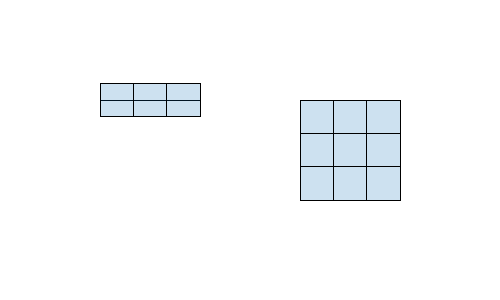
\includegraphics[width=0.7\textwidth]{figures/boxcounting-2.png}
    \caption{Box Counting - Cajas de lado $\frac{1}{3}$}
\end{figure}

\noindent Si utilizamos cajas más pequeñas, de lado $\frac{1}{3}$, vemos que para el segmento necesitamos $3$ y para el cuadrado $3^4$

\begin{figure}[H]
    \centering
    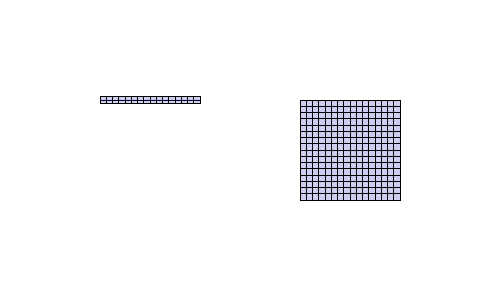
\includegraphics[width=0.7\textwidth]{figures/boxcounting-3.png}
    \caption{Box Counting - Cajas de lado $\frac{1}{n}$}
\end{figure}

\noindent Si continuamos con este proceso vemos que para el segmento necesitamos $n$ cajas de lado $\frac{1}{n}$ y para el cuadrado $n^2$\\

\noindent Vemos que el exponente es un buen indicador de la dimensión de los objetos. Si definimos $N(n)$ como el número de cajas de lado $\frac{1}{n}$ necesarias para cubrir el objeto, entonces tenemos que:

\begin{equation}
    N(n) = n^d
\end{equation}

\noindent Sacando logaritmos a ambos lados tenemos que:

\begin{equation}
    \log N(n) = \log n^d \Longleftrightarrow \log N(n) = d \log n \Longleftrightarrow d = \frac{\log N(n)}{\log n}
\end{equation}

\begin{definition}
    La dimensión de Minkowski-Bouligard de un conjunto $A$ es el límite de la expresión
    \begin{equation}
        \lim_{\epsilon \to 0} \frac{\log N(\epsilon)}{\log \frac{1}{\epsilon}}
    \end{equation}
    donde $N(\epsilon)$ es el mínimo de bolas de radio $\epsilon$ necesarias para recubrir el conjunto.
\end{definition}

\noindent Ahora vamos a ver que ocurre cuando intentamos calcular la dimensión de Minkowski-Bouligard de un fractal, como por ejemplo el triángulo de Sierpinski de base $1$.\\

\noindent Si intentamos cubrir el triángulo con cajas de lado $\frac{1}{2}$ vemos que necesitamos $4$ cajas.

\begin{figure}[H]
    \centering
    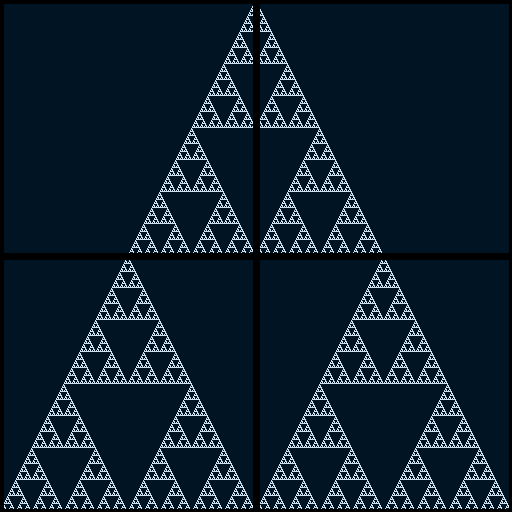
\includegraphics[width=0.5\textwidth]{figures/boxcounting-sierspinsky-1.png}
    \caption{Box Counting - Triángulo de Sierpinski - Cajas de lado $\frac{1}{2}$}
\end{figure}

\noindent Si utilizamos cajas más pequeñas, de lado $\frac{1}{4}$, necesitaremos $12$ cajas.

\begin{figure}[H]
    \centering
    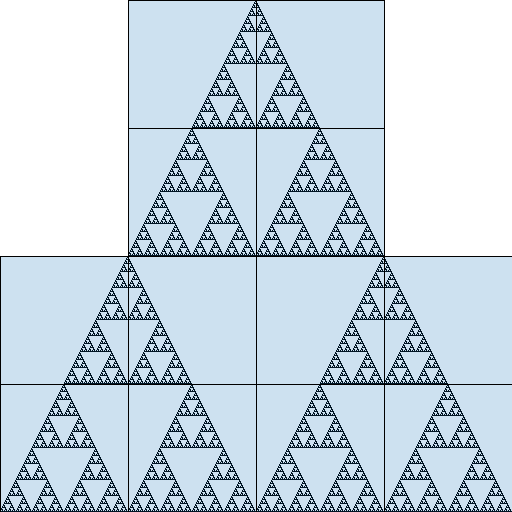
\includegraphics[width=0.5\textwidth]{figures/boxcounting-sierspinsky-2.png}
    \caption{Box Counting - Triángulo de Sierpinski - Cajas de lado $\frac{1}{4}$}
\end{figure}

\noindent Con cajas de lado $\frac{1}{8}$ necesitaremos $36$ cajas.

\begin{figure}[H]
    \centering
    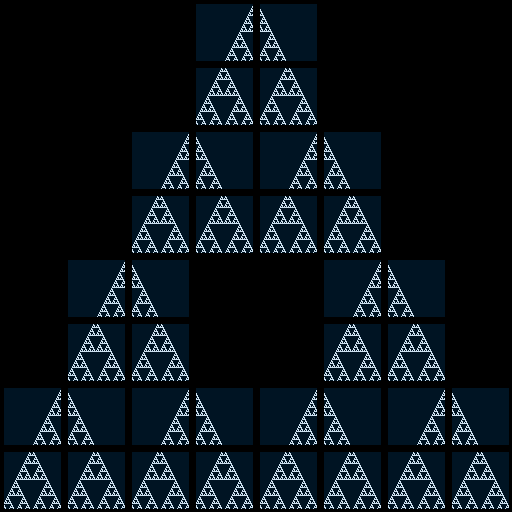
\includegraphics[width=0.5\textwidth]{figures/boxcounting-sierspinsky-3.png}
    \caption{Box Counting - Triángulo de Sierpinski - Cajas de lado $\frac{1}{8}$}
\end{figure}

\noindent Y con cajas de lado $\frac{1}{16}$ necesitaremos $108$ cajas.

\begin{figure}[H]
    \centering
    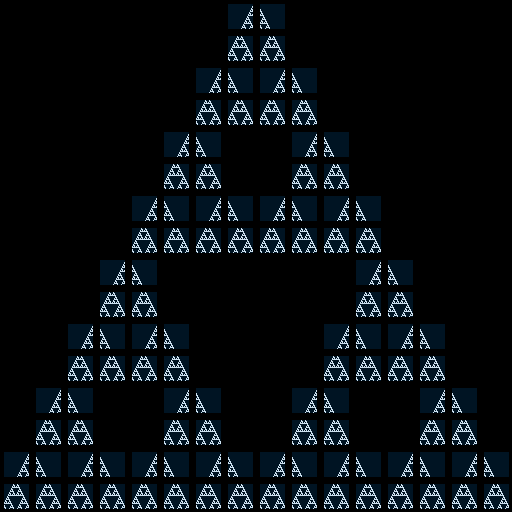
\includegraphics[width=0.5\textwidth]{figures/boxcounting-sierspinsky-4.png}
    \caption{Box Counting - Triángulo de Sierpinski - Cajas de lado $\frac{1}{16}$}
\end{figure}

\noindent Si continuamos con este proceso vemos que para el triángulo de Sierpinski necesitamos $4 \cdot 3^{n-1}$ cajas de lado $\frac{1}{2^n}$.
Si definimos $N(n)$ como el número de cajas de lado $\frac{1}{2^n}$ necesarias para cubrir el objeto, entonces tenemos que:

\begin{equation}
    \begin{split}
        & d = \lim_{n \rightarrow \infty} \frac{log (N(n))}{log (2^n)} = \lim_{n \rightarrow \infty} \frac{4 \cdot 3^{n-1}}{2^n} \approx \\
        & \approx \lim_{n \rightarrow \infty} \frac{3^n}{2^n} = \frac{\log{3}}{\log{2}} \approx 1.585\\
    \end{split}
\end{equation}

\noindent Como ya hemos comentado antes, nos sale un número real. Nuestra intuición nos sugiere que el triángulo de Sierpinski es \textit{"más que una curva"} pero \textit{"menos que una superficie"}\\
